%%%------------------------------------------------------------------------------------------------------------
\begin{tcolorbox}
[bicolor,sidebyside,width=12cm,righthand width=4cm,size=title,frame engine=empty,
 colback=blue!10!white,colbacklower=black!5!white]
 {\scriptsize
\begin{tabbing}
\texttt{XTensor w[3], e[3], h0, y;} \\
\texttt{XTensor C, H, d, U;} \\
\texttt{...}\\

\texttt{} \\
\texttt{for(unsigned i = 0; i < 3; i++)} \\
\texttt{\ \ \ \ e[i] = MMul(w[i], C);}\\
\texttt{e01 = Concatenate(e[0], e[1], -1);}\\
\texttt{e = Concatenate(e01, e[2], -1);}\\

\texttt{} \\
\texttt{h0 = TanH(MMul(e, H) + d);}\\
\texttt{y = Softmax(MMul(h0, U));}\\

\texttt{} \\
\texttt{for(unsigned k = 0; k < size; k++)\{} \\
\texttt{} \ \ \ \ ... // {\texttt{y}}的第$k$元素表示 $\textrm{P}(w|...)$\\
\texttt{} \ \ \ \ ... // $w$为词汇表里第$k$个词\\
\texttt{\}}

\end{tabbing}
}
\tcblower
\begin{center}
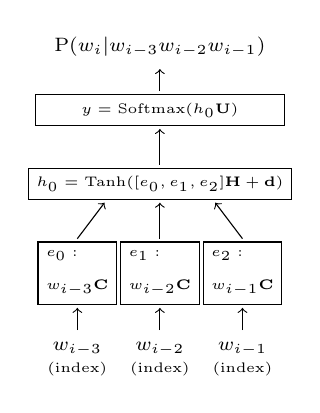
\begin{tikzpicture}
\begin{scope}
\node [anchor=west] (w0) at (0,0) {\scriptsize{$w_{i-3}$}};
\node [anchor=west] (w1) at ([xshift=0.5em]w0.east) {\scriptsize{$w_{i-2}$}};
\node [anchor=west] (w2) at ([xshift=0.5em]w1.east) {\scriptsize{$w_{i-1}$}};
\node [anchor=north] (index0) at ([yshift=0.5em]w0.south) {\tiny(index)};
\node [anchor=north] (index1) at ([yshift=0.5em]w1.south) {\tiny(index)};
\node [anchor=north] (index2) at ([yshift=0.5em]w2.south) {\tiny(index)};
\node [anchor=south,draw,inner sep=3pt,align=left] (e0) at ([yshift=1.0em]w0.north) {\tiny{$e_0:$}\\\tiny{$w_{i-3} \textbf{C}$}};
\node [anchor=south,draw,inner sep=3pt,align=left] (e1) at ([yshift=1.0em]w1.north) {\tiny{$e_1:$}\\\tiny{$w_{i-2} \textbf{C}$}};
\node [anchor=south,draw,inner sep=3pt,align=left] (e2) at ([yshift=1.0em]w2.north) {\tiny{$e_2:$}\\\tiny{$w_{i-1} \textbf{C}$}};
\node [anchor=south,draw,minimum width=9em,inner sep=3pt] (h0) at ([yshift=1.5em]e1.north) {\tiny{$h_0=\textrm{Tanh}([e_0,e_1,e_2] \textbf{H} + \textbf{d})$}};
\node [anchor=south,draw,minimum width=9em,inner sep=3pt] (h1) at ([yshift=1.5em]h0.north) {\tiny{$y=\textrm{Softmax}(h_0 \textbf{U})$}};
\node [anchor=south] (ylabel) at ([yshift=1em]h1.north) {\scriptsize{$\textrm{P}(w_i|w_{i-3}w_{i-2}w_{i-1})$}};

\draw [->] ([yshift=0.1em]w0.north) -- ([yshift=-0.1em]e0.south);
\draw [->] ([yshift=0.1em]w1.north) -- ([yshift=-0.1em]e1.south);
\draw [->] ([yshift=0.1em]w2.north) -- ([yshift=-0.1em]e2.south);
\draw [->] ([yshift=0.1em]e0.north) -- ([xshift=-2em,yshift=-0.1em]h0.south);
\draw [->] ([yshift=0.1em]e1.north) -- ([yshift=-0.1em]h0.south);
\draw [->] ([yshift=0.1em]e2.north) -- ([xshift=2em,yshift=-0.1em]h0.south);
\draw [->] ([yshift=0.1em]h0.north) -- ([yshift=-0.1em]h1.south);
\draw [->] ([yshift=0.1em]h1.north) -- ([yshift=-0.1em]ylabel.south);
\end{scope}
\end{tikzpicture}
\end{center}
\end{tcolorbox}
%%%------------------------------------------------------------------------------------------------------------

